\chapter{Конструкторский раздел}\label{sec:design}
\section{\protect\justifying\protect\RaggedRight Проектирование отношений сущностей}
Проектируемая база данных ориентирована на хранение информации, получаемой из web-приложения, содержащего систему оценки тональных прилагательных. Функционал приложения должен включать в себя регистрацию, авторизацию и возможность проставления оценок прилагательным. Соответственно, в базе данных можно выделить ряд сущностей. 
\begin{enumerate}
	\item Аккаунт хранит информацию, необходимую при регистрации -- электронная почта и пароль.
	\item Пользователь содержит информацию о личных характеристиках субъекта тональности -- национальность, возраст и гендерная принадлежность. 
	\item Населенный пункт -- это одна из характеристик субъекта тональности. Поскольку пользователь мог менять места проживания, связь этих двух сущностей -- <<многие ко многим>>.
	\item Место обучения -- сущность, содержащая характеристику об образовании, которое получает пользователь.
	\item Результат тестирования включает в себя оценку тонального прилагательного, присвоенная пользователем во время рабочей сессии. Возможные значения оценки -- числа от <<1>> до <<10>>.
	\item Тональное прилагательное.
\end{enumerate}
На рисунке \ref{fig:chen} приведена концептуальная схема проектируемой БД в нотации Чена. 
\begin{center}
	\begin{figure}[H]
		\centering
		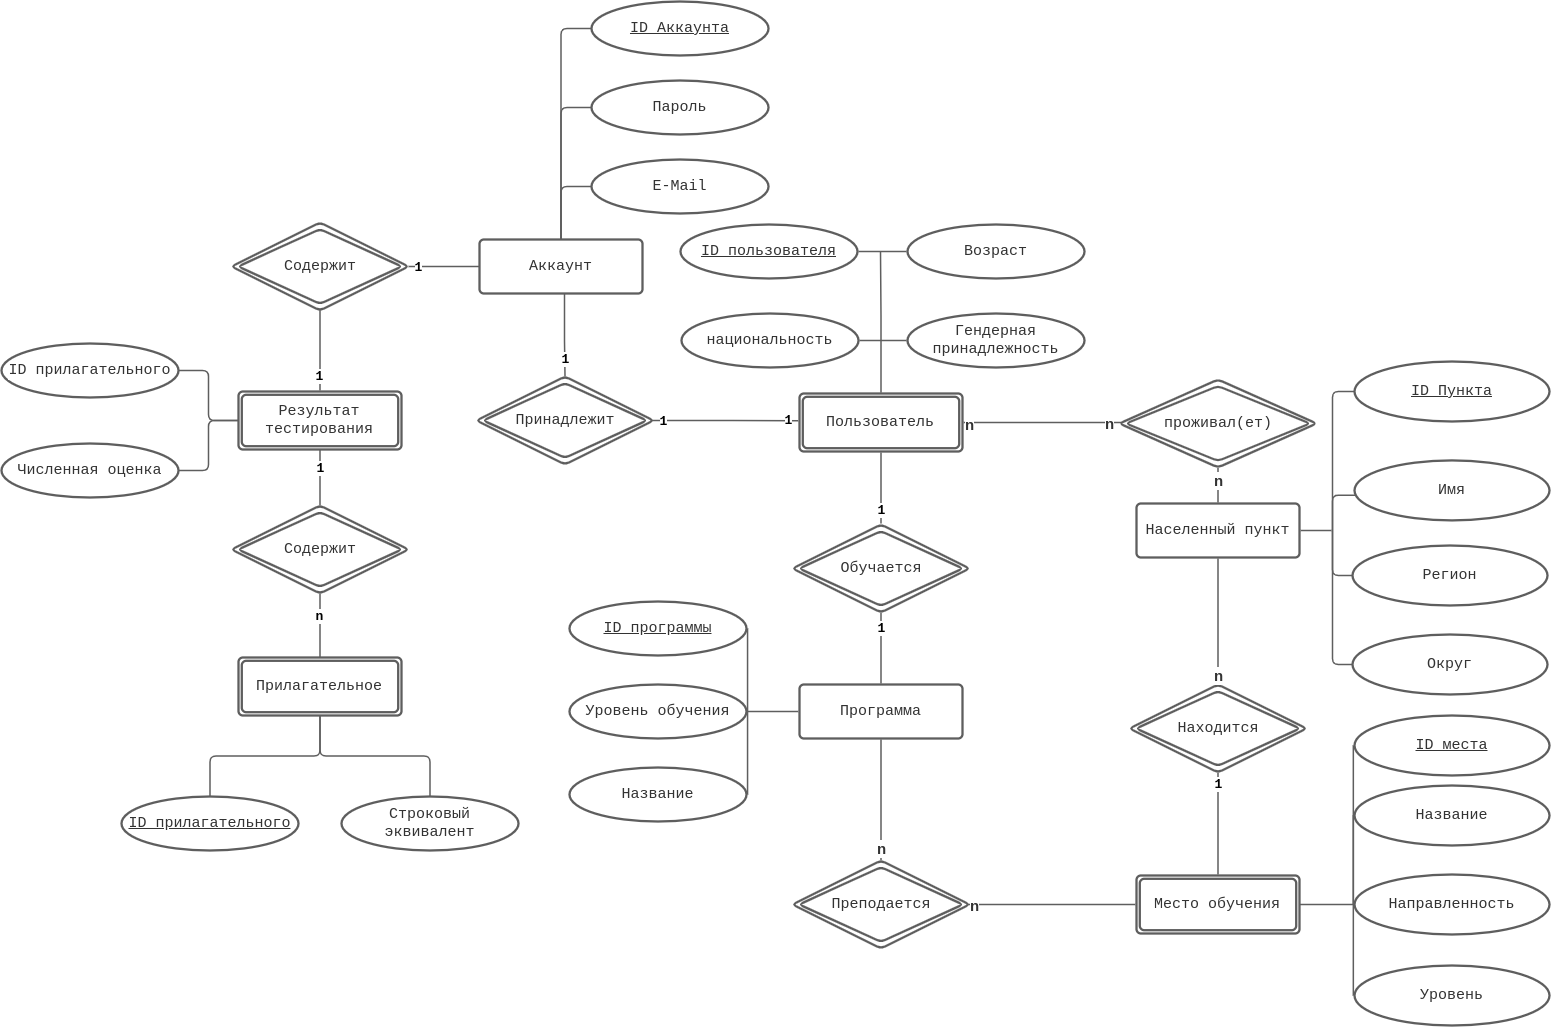
\includegraphics[width=\linewidth]{assets/term-chen.drawio.png}
		\caption{ER-диаграмма сущностей базы данных в нотации Чена}
		\label{fig:chen}
	\end{figure}
\end{center} 
\subsection{База данных Neo4j}
\section{Кеширование запросов к целевой БД}
\section{\protect\justifying\protect\RaggedRight Проектирование системы разметки интерфейса}
На рисунке \ref{fig:usecase} представлена диаграмма вариантов использования приложения. 

В системе выделены следующие группы участников: пользователь, зарегистрированный пользователь, администратор и модератор. Интерфейс незарегистрированного пользователя включает возможность регистрироваться и осуществлять вход в систему. После регистрации или авторизации интерфейс расширяется: опрашиваемый может проходить тестирование и смотреть свои результаты. 

Модератор может смотреть информацию о пользователях. Интерфейс администратора расширяет интерфейс модератора возможностью смотреть общую статистику.   
\begin{center}
	\begin{figure}[H]
		\centering
		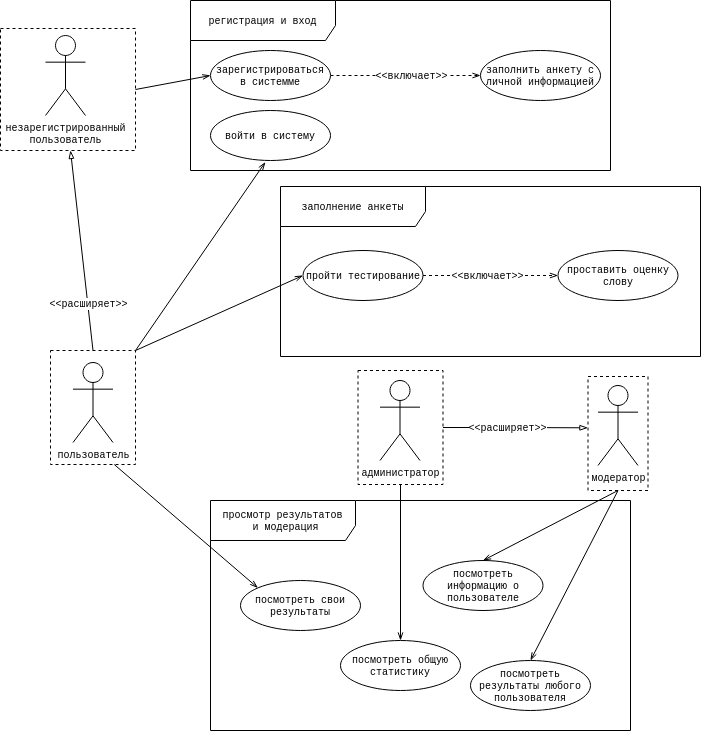
\includegraphics[width=0.85\linewidth]{assets/term-uc.drawio.png}
		\caption{Диаграмма вариантов использования системы}
		\label{fig:usecase}
	\end{figure}
\end{center}

Ниже представлена модель бизнес-процессов в нотации BPMN.

Бизнес-процесс состоит одного пула, поделенного на три дорожки --
\begin{center}
	\begin{figure}[H]
		\centering
		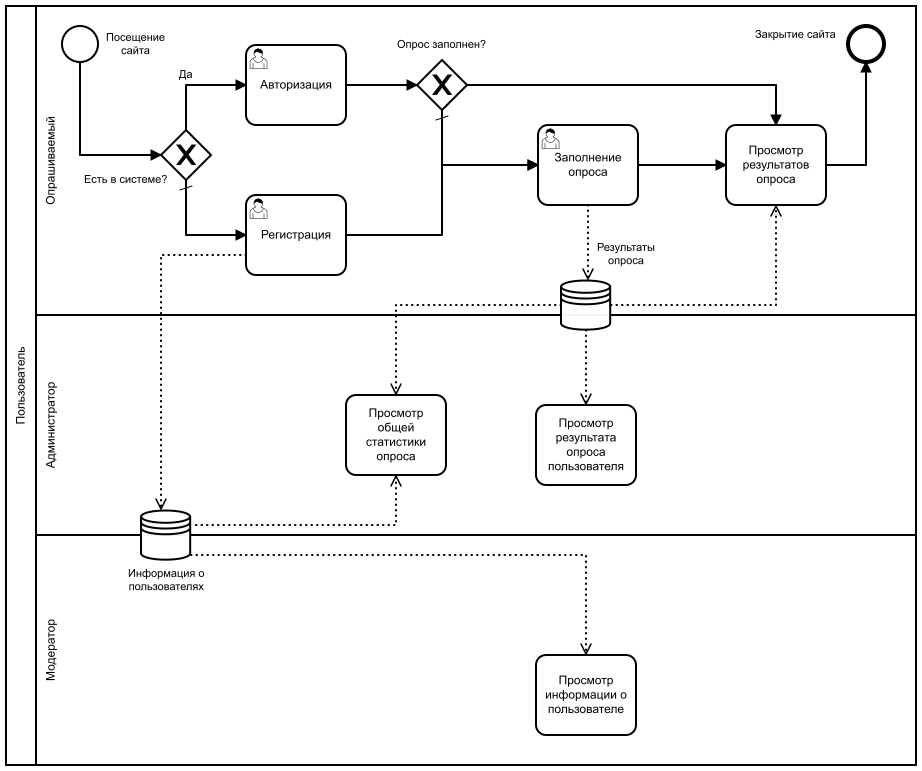
\includegraphics[width=\linewidth]{assets/term-bpmn.png}
		\caption{модель бизнес-процессов в нотации BPMN}
		\label{fig:bpmn}
	\end{figure}
\end{center}

\addsec{Вывод}
